\documentclass[a4paper]{report}
\usepackage[utf8]{inputenc}
\usepackage[T1]{fontenc} 
\usepackage[francais]{babel}
\usepackage{graphicx}
\usepackage{geometry}
\usepackage{color}
\usepackage{fancyhdr}
\pagestyle{fancy}
\fancyhf{}
\lhead{2011/2012}
\rhead{IUT Nancy Charlemagne}

\lfoot{Mathieu LEROUX}
\cfoot{Projet tuteuré: Déduplication \\ Licence ASRALL}
\rfoot{\thepage}
\renewcommand{\footrulewidth}{2pt}
\begin{document}
	\chapter*{Déduplication}
	La déduplication de données est une technique qui permet de minimiser de l'espace de stockage. Elle consiste à ne pas répliquer les données déja existantes sur le disque. Un fichier est décomposé sous forme de blocs de données car des fichiers peuvent avoir des blocs en commum. Le mécanisme de déduplication créé une table avec les indexs de tous les blocs de données des fichiers présent sur le disque. La taille des blocs peut varié selon les mécanismes utilisés mais plus les blocs sont petits, plus il y aura de chance qu'un autre bloc soit idendtique et donc, plus la déduplication sera efficace. En général, cette taille ne dépasse pas les 128ko.
 
 Quand un utilisateur dépose un fichier, le mécanisme crée ses indexs et regarde s'il n'y a pas des blocs déja existant. Si des blocs sont similaires alors une simple référence aux blocs déja existant sera créé. Le schéma ci-dessous montre comment la déduplication fonctionne. Les blocs étant de la meme couleur sont considérés identiques.\\
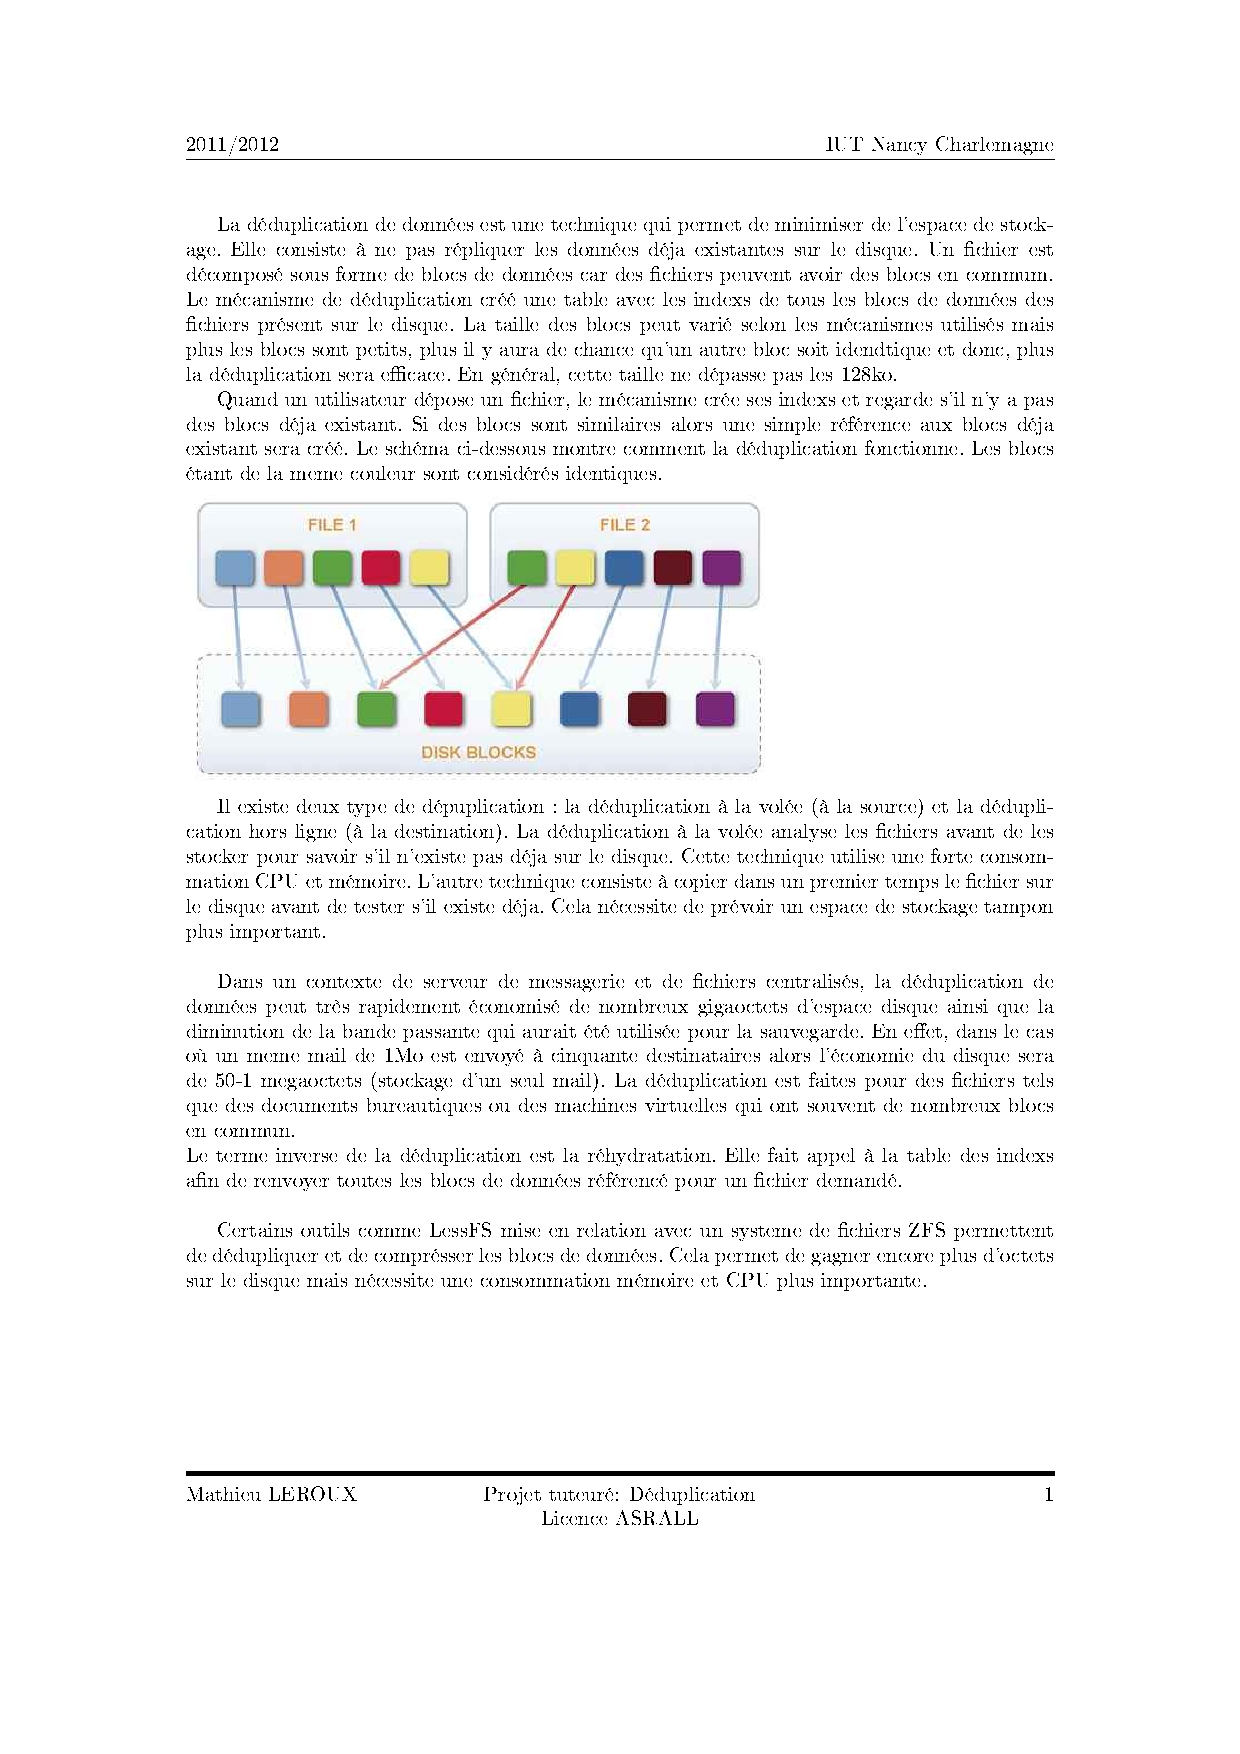
\includegraphics[width=10cm]{deduplication.jpg}

Il existe deux type de dépuplication: la déduplication à la volée (à la source) et la déduplication hors ligne (à la destination). La déduplication à la volée analyse les fichiers avant de les stocker pour savoir s'il n'existe pas déja sur le disque. Cette technique utilise une forte consommation CPU et mémoire. L'autre technique consiste à copier dans un premier temps le fichier sur le disque avant de tester s'il existe déja. Cela nécessite de prévoir un espace de stockage tampon plus important. \\

Dans un contexte de serveur de messagerie et de fichiers centralisés, la déduplication de données peut très rapidement économisé de nombreux gigaoctets d'espace disque ainsi que la diminution de la bande passante qui aurait été utilisée pour la sauvegarde. En effet, dans le cas où un meme mail de 1Mo est envoyé à cinquante destinataires alors l'économie du disque sera de 50-1 megaoctets (stockage d'un seul mail). La déduplication est faites pour des fichiers tels que des documents bureautiques ou des machines virtuelles qui ont souvent de nombreux blocs en commun.\\
Le terme inverse de la déduplication est la réhydratation. Elle fait appel à la table des indexs afin de renvoyer toutes les blocs de données référencé pour un fichier demandé.\\

Certains outils comme LessFS mise en relation avec un systeme de fichiers ZFS permettent de dédupliquer et de comprésser les blocs de données. Cela permet de gagner encore plus d'octets sur le disque mais nécessite une consommation mémoire et CPU plus importante.

	\chapter*{Compression}
	Tout comme la déduplication, la compression est une technique qui permet d'économiser de l'espace de stockage. Chaque fichier est constitué d'une succession de millions de bits 0 ou 1. La compression permet de diminuer le nombre de bit que constitue un fichier en changeant la succession de bit de depart. Suivant l'algorithme de codage utiliser, le taux de compression peut differer. Les algorithme d'encodage sont plus ou moins efficace selon le type de fichier compresser.\\
 Il existe deux types de compression: la compression avec perte et sans perte. La compression sans perte signifie qu'après la décompression, le fichier sera identique au fichier compressé. C'est le plus souvent utilisé sur des documents, des fichiers executables ou des archives. Ces données étant principalement des caractères texte, ils ne peuvent pas etre modifier. Les formats de documentation tel que txt,doc ou pdf sont donc compresser sans perte.  Tant qu'à la compression avec perte, les fichiers décompréssé ne seront pas exactement identique au fichier original mais les informations seront sensiblement les memes. Les types de fichiers utilisés par cette compression sont les images, les sons et les vidéos. Cett technique se repose sur la limitation des sens de l'homme comme la vision et l'audition. L'homme ne pourra donc pas identifier les différences du fichier original que du fichier après décompressage. Les formats de fichiers jpeg, avi ou mp3 sont donc compresser avec pertes. \\(
Pour chaque technique de compression, il existe plusieurs algorithme de codage.\\
	\section{Compression sans perte}
	Parmis les algorithmes sans pertes, il y a les algorithmes tel que Lempei-Ziv où le codage RLE (Run-Length Encoding) qui consistent à remplacer des suites de bits utilisées plusieurs fois dans un même fichier. D'autres algorithme comme l'algorithme de codage Huffman détermine les suites de bit et plus une suite est utilisée souvent, plus la suite qui la replacera sera courte.
	\subsection{L'algorithme Lempel-Ziv}
		Cet algorithme se divise en deux versions distinctes : LZ77 et LZ78. Ces algorithmes utilisent un dictionnaire où ils référencent les motifs récurrents. A la rencontre d'un motif du dictionnaire, une simple référence au motif est fait (fenêtre glissante). La déduplication utilise globalement le meme procédé.\\
	\subsubsection{LZ77}
		La compression LZ77 encode avec un taux de compression inferieur à d'autres algorithmes comme PPM et CM (voir ci-dessous) mais a le double avantage d'être rapide et asymetrique. Cela lui permet d'utiliser un algorithme de décompression différent que celui de la compression. Ainsi, la compression pourra etre rapide et la décompression performante. Les variantes LZSS et LZMA sont basées sur la compression LZ77 et supprime quelques inconvénients de celle-ci tel que le taux de compression assez faible (pour LZMA) ou le probleme si aucun motif récurrent n'est rencontré (pour LZSS). Ce problème aura pour consequence d'augmenter la taille du fichier. La compression LZ77 est la base des algorithmes comme Deflate (ZIP, gzip) et donc LZMA (7-zip).
	\subsubsection{LZ78}
		La compression LZ78 ou Lempel-Ziv-Welch utilise aussi un dictionnaire mais au lieu de le remplir au fur et à mesure des motifs rencontré, il crée un dictionnaire initial de tous les symboles possibles. Cela permet d'ameliorer la compression car les données du dictionnaire ne devant plus etre envoyées au décompresseur, l'espace utilisé est réduit. L'utilisation de cette technique a été réduite jusque 2003 car elle a été brevetée par UNISYS qui n'avait pas laissé la licence libre.
	\subsubsection{LZO}
		Lempel-Ziv-Oberhumer (LZO) est un algorithme de compression en temps réel se basant sur les dictionnaires. Ces avantages sont une compression et décompression rapide. L'un des logiciels l'utilisant est lzop.
	\subsection{L'algorithme RLE}
		Le run-length encoding (codage par plages) est une technique de compression qui s'applique uniquement sur des documents scannés en noir et blanc tel que des fax. Elle consiste à factoriser les termes d'une meme couleur. Ainsi la chaine : NNNNNNNBBBBNNNNNNNNNNBB (N etant le nombre de points noir et N etant le nombre de points blanc) sera encodé par RLE en : 7N4B10N2B . Les formats d'images utilisent cette compression en considérant que toutes les lignes de pixels sont jointes pour former une unique séquence de couleur. Les images BMP utilisent cette compression en 1,4 et 8 bits/pixel (noir et blanc, 16 couleurs et 256 couleurs). Le format PCX utilise aussi cette compression pour les images de 8 et 24 bits/pixels. Celles de 24 bits étant découpé en trois parties de 8 bits chacunes.
	\subsection{Codage par modélisation de contexte}
	\subsubsection{Prédiction par reconnaissance partielle (PPM)}
		La prédiction par reconnaissance partielle se base sur une modélisation de contexte pour évaluer la probabilité des différents symboles. Le contexte est un ensemble de symboles déja rencontrés dans la source de données. Elle utilise les données déja analysés pour en déduire les données à analyser. Ainsi plus le contexte est long, meilleur sera la prediction et donc la compression. La prédiction obtenue servira d'entrée à un codage entropique comme le codage Huffman. Elle a l'avantage d'etre l'une des plus performantes sur la compression de fichiers texte mais a l'inconvénient de consommer enormément de mémoire si le contexte est très grand. La PPM est un algorithme symétrique contrairement à Lempel-Ziv ce qui signifie qu'il utilise le meme pour la compression que pour la décompression. Cela implique un temps d'execution identique et assez lent.
	\subsubsection{Pondération de contextes (CM)}
		La pondération de contextes consiste à utiliser plusieurs prédicteurs (par exemple des PPM) pour obtenir l'estimation la plus fiable possible du symbole à venir. A l'image de la prédiction par reconnaissance partielle, les taux de compressions sont très élevés mais proportionnellemnt aussi lente que la taille du contexte.
	\subsection{L'algorithme de codage Huffman}
		Cette compression s'apparente à la compression du code morse. Elle consiste donc à coder les séquences fréquentes sur peu de place et ce qui revient rarement sur des séquences plus longue. L'inconvénient avec ce procédé c'est qu'il faut avoir analysé tout le fichier pour créer une table avec les redondances avant de pouvoir compresser. Il faut donc envoyer la table pour pouvoir le décompresser ce qui peut etre problematique quand le fichier a compressé est petit. Le codage Huffman adaptatif corrige ce problème car il remplit au fur et à mesure la table et démarre la compression avec une table de base. \\
	Ce codage est utilisé en seconde compression après que le premier algorithme (tel que LZ77) est mise en evidence la redondance d'information que ce codage peut compresser. Ce codage peut etre utilise pour la compression tel que JPEG, MPEG ou MP3 où les données inperceptibles par l'homme sont supprimées mais on parle donc de compression avec pertes.
	\section{Compression avec pertes}

         
\end{document} 
